\documentclass[12pt]{amsart}
% packages
\usepackage{graphicx}
\usepackage{setspace}
\usepackage{amssymb,amsmath,amsthm,amsfonts,amscd}
\usepackage{hyperref}
\usepackage{color}
\usepackage{booktabs}
\usepackage{tabularx}
\usepackage{enumitem}
\usepackage[retainorgcmds]{IEEEtrantools}
\usepackage[notref,notcite,final]{showkeys}
\usepackage[final]{pdfpages}
\usepackage{fancyhdr}
\usepackage{upgreek}
\usepackage{multicol}
% set margin as 0.75in
\usepackage[margin=0.75in]{geometry}

% tikz-related settings
\usepackage{tikz}
\usepackage{tikz-cd}
\usetikzlibrary{cd}

% theorem environments with italic font
\newtheorem{thm}{Theorem}[section]
\newtheorem*{thm*}{Theorem}
\newtheorem{lemma}[thm]{Lemma}
\newtheorem{prop}[thm]{Proposition}
\newtheorem{claim}[thm]{Claim}
\newtheorem{corollary}[thm]{Corollary}
\newtheorem{conjecture}[thm]{Conjecture}
\newtheorem{question}[thm]{Question}
\newtheorem{procedure}[thm]{Procedure}
\newtheorem{assumption}[thm]{Assumption}

% theorem environments with roman font (use lower-case version in body
% of text, e.g., \begin{example} rather than \begin{Example})
\newtheorem{Definition}[thm]{Definition}
\newenvironment{definition}
{\begin{Definition}\rm}{\end{Definition}}
\newtheorem{Example}[thm]{Example}
\newenvironment{example}
{\begin{Example}\rm}{\end{Example}}

\theoremstyle{definition}
\newtheorem{remark}[thm]{\textbf{Remark}}

% special sets
\newcommand{\A}{\mathbb{A}}
\newcommand{\C}{\mathbb{C}}
\newcommand{\F}{\mathbb{F}}
\newcommand{\N}{\mathbb{N}}
\newcommand{\Q}{\mathbb{Q}}
\newcommand{\R}{\mathbb{R}}
\newcommand{\Z}{\mathbb{Z}}
\newcommand{\cals}{\mathcal{S}}
\newcommand{\ZZ}{\mathbb{Z}_{\ge 0}}
\newcommand{\cala}{\mathcal{A}}
\newcommand{\calb}{\mathcal{B}}
\newcommand{\cald}{\mathcal{D}}
\newcommand{\calh}{\mathcal{H}}
\newcommand{\call}{\mathcal{L}}
\newcommand{\calr}{\mathcal{R}}
\newcommand{\la}{\mathbf{a}}
\newcommand{\lgl}{\mathfrak{gl}}
\newcommand{\lsl}{\mathfrak{sl}}
\newcommand{\lieg}{\mathfrak{g}}

% math operators
\DeclareMathOperator{\kernel}{\mathrm{ker}}
\DeclareMathOperator{\image}{\mathrm{im}}
\DeclareMathOperator{\rad}{\mathrm{rad}}
\DeclareMathOperator{\id}{\mathrm{id}}
\DeclareMathOperator{\hum}{[\mathrm{Hum}]}
\DeclareMathOperator{\eh}{[\mathrm{EH}]}
\DeclareMathOperator{\lcm}{\mathrm{lcm}}
\DeclareMathOperator{\Aut}{\mathrm{Aut}}
\DeclareMathOperator{\Inn}{\mathrm{Inn}}
\DeclareMathOperator{\Out}{\mathrm{Out}}
\DeclareMathOperator{\Gal}{\mathrm{Gal}}


% frequently used shorthands
\newcommand{\ra}{\rightarrow}
\newcommand{\se}{\subseteq}
\newcommand{\ip}[1]{\langle#1\rangle}
\newcommand{\dual}{^*}
\newcommand{\inverse}{^{-1}}
\newcommand{\norm}[2]{\|#1\|_{#2}}
\newcommand{\abs}[1]{\lvert #1 \rvert}
\newcommand{\Abs}[1]{\bigg| #1 \bigg|}
\newcommand\bm[1]{\begin{bmatrix}#1\end{bmatrix}}
\newcommand{\op}{\text{op}}

% nicer looking empty set
\let\oldemptyset\emptyset
\let\emptyset\varnothing

\setlist[enumerate,1]{topsep=1em,leftmargin=1.8em, itemsep=0.5em, label=\textup{(}\arabic*\textup{)}}
\setlist[enumerate,2]{topsep=0.5em,leftmargin=3em, itemsep=0.3em}


%pagestyle
%\pagestyle{fancy} 

\begin{document}
\begin{center}
    \textsc{Linear Algebra. HW 1\\ Ian Jorquera}
\end{center}
\vspace{1em}

\begin{itemize}
\item[(1)] % 
We could create a table with relations on top and points on the side. With an entry for $(x,\ell)$ being 1 if the relation is satisfied and zero if it is not.\\

\item[(2)]
We will show that $\R^2$ is an affine plane with the incidence system as described.
Let $\vec{u},\vec{v}\in \R^2$ be vectors, we will then define $\ell_{\vec{u},\vec{v}}:=\{t\cdot \vec{u}+\vec{v}|t\in\R\}$. Notice first that for any points $\vec{u},\vec{v}\in \R^2$ that the line $\ell_{\vec{u}-\vec{v},\vec{v}}$ contains both vectors $\vec{u}$ and $\vec{v}$, at $t=1$ and $t=0$ respectively. Furthermore for any point $\vec x\in \ell_{\vec{u}, \vec{v}}$ we have that $\ell_{\vec{u}, \vec{v}}=\ell_{\vec{u}, \vec{x}}$. To see this let $w\in \ell_{\vec{u}, \vec{v}}$ and notice that there exists some $t,t'\in \R$ such that $t\cdot \vec{u}+\vec{v}=\vec{x}$ and $t'\cdot \vec{u}+\vec{v}=\vec{w}$. Notice that this means $\vec{w}=t'\cdot \vec{u}+\vec{v}=t'\cdot \vec{u}+\vec{x}-t\cdot \vec{u}=(t'-t)\cdot \vec{u}+\vec{x}$, so $\vec{w}\in\ell_{\vec{u},\vec{x}}$. Now let $\vec{w}\in\ell_{\vec{u},\vec{x}}$ which means that there exists some $t'\in \R$ such that $\vec{w}=t'\cdot \vec{u}+\vec{x}=t'\cdot \vec{u}+t\cdot \vec{u}+\vec{v}=(t'+t)\vec{u}+\vec{v}$, so $\vec{w}\in \ell_{\vec{u},\vec{v}}$. So $\ell_{\vec{u},\vec{v}}=\ell_{\vec{u},\vec{x}}$. \\

Now assume that $\vec{x},\vec{y}$ are distinct vectors on the line $\ell_{\vec{u},\vec{v}}$ for some vectors $\vec{u},\vec{v}$. We know that $\vec{x}$ and $\vec{y}$ also exist on the line $\ell_{\vec{y}-\vec{x},\vec{x}}$ by the above properties. 
And by the above properties we know that $\ell_{\vec{u},\vec{v}}=\ell_{\vec{u},\vec{x}}$. Furthermore we know 
that there exists $t_1,t_2\in \R$ such that $\vec{x}=t_1\cdot \vec{u}+\vec{v}$ 
and $\vec{y}=t_2\cdot \vec{u}+\vec{v}$, meaning $\vec{y}-\vec{x}=(t_2-t_1)\vec{u}$ which is 
a scalar multiple of $u$ so by refactoring $t$ we know that $\ell_{\vec{y}-\vec{x},\vec{x}}=\ell_{\vec{u},\vec{x}}=\ell_{\vec{u}, \vec{v}}$.
This proves (1), as any two points $\vec{x},\vec{y}$ determine the unique line $\ell_{\vec{y}-\vec{x},\vec{x}}$\\

Now assume that $\vec{w}\not\in \ell_{\vec{u},\vec{v}}$ for vectors $\vec{u},\vec{v},\vec{w}\in \R^2$. Notice that the line $\ell_{\vec{u}, \vec{w}}$ shares no points with $\ell_{\vec{u},\vec{v}}$. To see this assume there was an intersection point, meaning for some $t_1,t_2\in \R$ that $t_1\cdot \vec{u}+\vec{v}=t_2\cdot\vec{u}+\vec{w}$, which would mean $(t_1-t_2)\cdot \vec{u}+\vec{v}=\vec{w}\in\ell_{\vec{u},\vec{v}}$, a contradiction. To see that this line is unique assume there exits another line $\ell_{u',w}$ that contains $w$. Assume that $u\neq u'$. In which case notice that they span all of $\R^2$ and therefore there exists a linear combination that equals the point $v-w$ and so $\ell_{u',w'}$ and $\ell_{\vec{u},\vec{v}}$ intersect and are not parallel. So $\ell_{\vec{u},\vec{v}}$ is unqiue.

Notice that for any line $\ell_{\vec{u},\vec{v}}$ for vectors $\vec{u},\vec{v}\in \R^2$ we have that $\vec{v}\in \ell_{\vec{u},\vec{v}}$, for $t=0$ and $\vec{u}+\vec{v}\in\ell_{\vec{u},\vec{v}}$, for $t=1$. This proves (3).\\

Consider the vectors $(0,1), (1,0)$, and $(1,1)$. Notice that there exists no $t$ such that $(1,1)=t\cdot ((1,0)-(0,1))+(1,0)$. So these points are non-colinear.\\


\item[(3)]
For 4 points we may have the affine geometry
\begin{center}
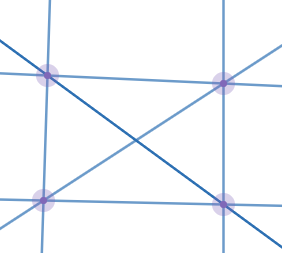
\includegraphics[scale=.4]{affinegeom4pt.PNG}
\end{center}
And for $9$ points we may have the affine geometry shown below
\begin{center}
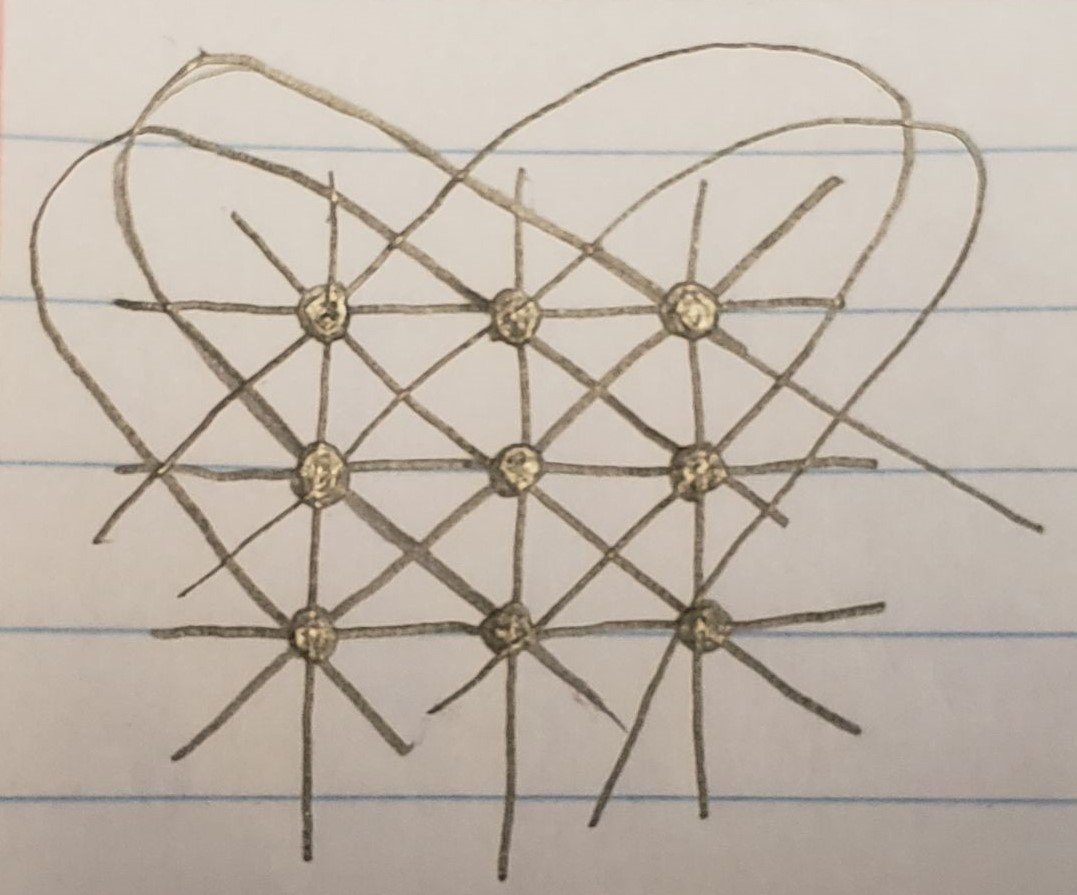
\includegraphics[scale=.15]{affinegeom9pt.jpg}
\end{center}

\item[(4)]
Consider an affine geometry with three points labeled $1$, $2$ and $3$. We know these three points would exist on at least one common plane. So we may assume that our three points are an affine plane. Notice that WLOG we would necessarily have a line between $1$ and $2$, which we will call $\ell$. And now because an affine plane has three non-collinear points we know that $3$ is not on the line $\ell$. In this case we would also necessarily have lines between $1$ and $3$ and $2$ and $3$. These would be the only three lines as from problem 2, two points determine a line. This means we do not satisfy condition $2$ as there does not exist a line containing $3$ that does not intersect with $\ell$.\\

5 points also can not form an affine geometry. Assume there was an affine geometry with $5$ points. From problem $6$ we know that all lines will have the same number of points. If all lines had $5$ points there would be no subset of $3$ non-colinear points, and so would not be an affine geometry. if all lines had $4$ points then any two lines would have to share $3$ points which break condition (1). If every line had $3$ points then every two lines would intersect at $1$ points and therefore there would be no parallel lines, and therefore does not satisfy condition (2). Finally consider the case where every line has $2$ points. WLOG call the points $1,2,3,4$ and $5$. We know by (1) that there must be the lines $\ell_{1,2}$ and $\ell_{3,4}$ which are parallel. Furthermore there must be the line $\ell_{4,5}$ and $\ell{3,5}$ which are both parallel with $\ell_{1,2}$. However this break condition (2).\\

\item[(5)] Let $\ell$ be a parallel line. Notice that $\ell$ must be parallel with its self as it shares all its points with its self. So parallel is reflexive. Now for a second line $\ell'$, assume that $\ell||\ell'$. This means that if $\ell$ has one point in common with $\ell'$ then $\ell$ and $\ell'$ must have all their points in common. Notice that if $\ell'$ has one point in common with $\ell$ then $\ell$ has one point in common with $\ell'$ so $\ell$ and $\ell'$ must have all their points in common. So parallel is symmetric.

Finally consider a third line $\ell^*$. And assume that $\ell||\ell'$ and $\ell'||\ell^*$. And suppose that $\ell$ and $\ell^*$ are not parallel, meaning they share at least $1$ points but not all(which means they share exactly one point as sharing two points would mean they are the same line). Let $w\in \ell\cap\ell^*$ be this point. first assume that WLOG $\ell$ and $\ell'$ share a point, and therefore all their points. This means that $\ell=\ell'$ which is parallel to $\ell^*$, but because they share the point $w$ we know that $\ell=\ell'=\ell^*$, which is a contradiction. Now assume that $\ell$ and $\ell'$ share no points In this case we know that $w\not\in \ell'$ and by axion 2 of affine planes there exists a distinct line containing this point that shares no points with $\ell'$. This line is $\ell=\ell^*$(as both lines satisfy the axiom 2 requirement).\\

\item[(6)] Let $\ell$ and $\ell'$ be two parallel lines. If they share a point then they then share all their points meanings the identity map on the points is a bijection between lines. Otherwise if they share no points in common let $u\in \ell$ and $w\in \ell'$. There exists, by axiom (1) a distinct line containing $u$ and $w$. Now consider the map $f:\ell\ra\ell'$ where $f$ maps a point $p\in\ell$ ($p\neq u$) to $q\in\ell'$ such that $q$ is the intersection between $\ell'$ and $\ell^*$, where $\ell^*$ is the line guaranteed by axiom 2 when considering the line $\ell_{u,w}$ and the point $p$. And $u\mapsto w$. Notice that for any point $q\in\ell'$ there exists the distinct line $\ell^*$ from axiom 2 when considering the line $\ell_{v,w}$ and the point $q$. This line must intersect $\ell$ at a point $p$, where $f(p)=q$. So $f$ is surjective. Furthermore we can construct a function $g:\ell'\ra\ell$ that maps points along the same line $\ell^*$ guaranteed from axiom 2. This function is an inverse for $f$. Notice that for $p\in\ell$ (and the point it maps to $q$) that $g(f(p))=g(q)=p$ and for $q\in\ell'$ (and the point it maps to $p$) that $f(g(q))=f(p)=q$. So parallel lines have the same number of points.\\

\item[(7)]

 Let $\ell$ and $\ell'$ be two lines that intersect at a single point $x$. let $u\in \ell$ and $w\in \ell'$ such that $u\neq x$ and $w\neq x$. There exists, by axiom (1) a distinct line containing $u$ and $w$. Now consider the map $f:\ell\ra\ell'$ where $f$ maps a point $p\in\ell$ ($p\neq u$) to $q\in\ell'$ such that $q$ is the intersection between $\ell'$ and $\ell^*$, where $\ell^*$ is the line guaranteed by axiom 2 when considering the line $\ell_{u,w}$ and the point $p$. And $u\mapsto w$. Notice that for any point $q\in\ell'$ there exists the distinct line $\ell^*$ from axiom 2 when considering the line $\ell_{v,w}$ and the point $q$. This line must intersect $\ell$ at a point $p$, where $f(p)=q$. So $f$ is surjective. Furthermore we can construct a function $g:\ell'\ra\ell$ that maps points along the same lines $\ell*$ guaranteed from axiom 2. This function is an inverse for $f$. Notice that for $p\in\ell$ (and the point it maps to $q$) that $g(f(p))=g(q)=p$ and for $q\in\ell'$ (and the point it maps to $p$) that $f(g(q))=f(p)=q$. So parallel lines have the same number of points.\\

 Any two lines $\ell$ and $\ell'$ either share no points, share $1$ point or share all their points, and by problem 6 and 7 we know that in any of these case $\ell$ and $\ell'$ would have a bijection between their points.\\

 \item[(8)]
A plane through the origin can be represented by linear combinations of any two distinct vectors. So we will denote a plane in $\R^3$ as $p_{\vec{u},\vec{v}}=span\{u,v\}=\{ut+vr|t,r\in\R\}$. Similarly a line through the origin is determined by a single vector that spans it. so $\ell_{\vec{u}}=span\{u\}=\{ut|t\in\R\}$. Now let $\ell_u$ and $\ell_v$ be distinct points in $\R^3$. Notice that because they are distinct $u$ and $v$ are linearly independent and determine the plane $p_{u,v}$.\\ 

Now consider any two lines $p_{u,v}$ and $p_{u',v'}$ We can determine their normal vectors $n,n'$ by taking the cross product of the vectors that determine them. At which point we know that the cross product of the normal vectors $n\times n'$, which is a vector determines the point that the lines intersect. Notice that $(n\times n')\cdot n=0=(n\times n')\cdot n'$ meaning $(n\times n')$ exists on both lines and $\ell_{n\times n'}$ is therefore the intersection.\\

Notice that no three of the points $\ell_{(1,0,0)}$, $\ell_{(0,1,0)}$, $\ell_{(0,0,1)}$ and $\ell_{(1,1,1)}$ are collinear.\\

\item[(9)] Let $\ell$ and $\ell'$ be two lines in a protective plane $P$. We can turn $P$ into an affine geometry $A$ by removing a hyperplane, and in the case of protective plane, a hyperplane would be a line. So let $A$ be the affine plane that is the result of removing any line other then $\ell$ or $\ell'$. In $A$ the two lines $\ell$ and $\ell'$ share the same number of points. Notice that in $P$ $\ell$ and $\ell'$ would have one addition point each, the intersection with the removed hyperplane. So $\ell$ and $\ell'$ share the same number of points.
\end{itemize}

\end{document}


